\appendix
\addcontentsline{toc}{chapter}{Appendix} % adds an entry to the table of contents

\chapter{Data collection}

\section{Cantonal data sources}

\subsection*{Parcel boudaries}
\label{app:canton_parcels}

 [ADD FIGURE ON THE AVAILABILITY OF THE DATA]
 
  [ADD TABLE ON THE SOURCES OF THE DATA]

\section{Data pre-processing}

\subsection*{Missing data in the RBD}
\label{app:rbd}
[DEMAND MAPPING LATEX DOCUMENT CONTAINS SOME INFORMATION]

\subsection*{Sub-sectors of industrial and service sectors}
\label{app:noga}

To link the STATENT data (Section \ref{data_rbd_statent}) to different economic activities and to estimate their heat and electricity demand, we use a grouping of NOGA codes into sub-sectors of service and industrial sector based on the mapping suggested in the analysis of the energy use in the industry and services sectors (2019) \cite{bfe_energieverbrauch_2019}, as shown in Table~\ref{tab:noga}. Some NOGA codes are not assigned to any sector, as these codes are considered to have no or a negligible demand for energy and are hence not relevant for the estimation of energy demand (Section \ref{demand_chapter}).

\begin{table}[ht]
\centering
\footnotesize
\caption{Mapping of NOGA codes to sub-sectors of the industry and service sectors}
\label{tab:noga}

\resizebox{\textwidth}{!}{%
\begin{tabular}{llll}
\hline
\textbf{Sector}            & \textbf{Sub-sector}        & \textbf{Sector ID \cite{bfe_energieverbrauch_2019}} & \textbf{NOGA-Code}                                   \\ \hline
\multirow{12}{*}{Industry} & Food production            & 1                            & 10-12                                                \\
                           & Textile / Leather          & 2                            & 13-15                                                \\
                           & Paper / Print              & 3                            & 17, 18                                               \\
                           & Chemistry / Pharmaceutical & 4                            & 20, 21                                               \\
                           & Cement / Concrete          & 5                            & -                                                    \\
                           & Other non-ferrous minerals & 6                            & 23                                                   \\
                           & Metal / Iron               & 7                            & 24                                                   \\
                           & Non-ferrous metals         & 8                            & -                                                    \\
                           & Metal / Tools              & 9                            & 25,27                                                \\
                           & Machines                   & 10                           & 28                                                   \\
                           & Other industries           & 11                           & 7-9, 16, 22, 29-32                                   \\
                           & Construction               & 12                           & 41-43                                                \\ \hline
\multirow{7}{*}{Services}  & Trade                      & 13                           & 45-47, 95                                            \\
                           & Hospitality                & 14                           & 55, 56                                               \\
                           & Credit / Assurances        & 15                           & 64-66                                                \\
                           & Administration             & 16                           & 84                                                   \\
                           & Schools                    & 17                           & 85                                                   \\
                           & Health / Welfare           & 18                           & 75, 86-88                                            \\
                           & Other services             & 19                           & 33, 36-39, 49-53, 58-63, 68-74, 77-82, 85, 90-94, 96 \\ \hline
\end{tabular}%
}
\end{table}

\subsection*{Roads and railways}
\label{app:roads}

To convert roads and railways of the TLM into vector polygons, they are buffered by their width. While road widths are defined for some roads, it has to be derived for several other road objects. We use high-resolution overhead imagery for Switzerland in combination with the TLM and geospatial tools to identify street patterns and measure the typical width for different road and railways types. The resulting mapping between road and railway objects and their width is shown in Table~\ref{tab:roads}.  

\begin{table}[ht]
\centering
\footnotesize
\caption{Mapping of road and railway widths to road types provided in the TLM.}
\label{tab:roads}

\begin{tabular}{llll}
\hline
\textbf{Type}            & \textbf{Description}    & \textbf{Object ID(s) \cite{swisstopo_swisstlm3d_2018}} & \textbf{Width (m)} \\ \hline
\multirow{5}{*}{Road}    & Driveways           & 0, 1, 5, 6                      & 6                  \\
                         & Connecting roads    & 4                               & 6                  \\
                         & Road (3,4,6,8,10 m) & 8-11, 20                        & 3-10*              \\
                         & Regional road       & 21                              & 15                 \\
                         & Highway             & 2                               & 30                 \\ \hline
\multirow{3}{*}{Railway} & Normal track        & 0                               & 5                  \\
                         & Narrow track        & 2, 4                            & 3                  \\
                         & Small train         & 5                               & 3                  \\ \hline
\multicolumn{4}{l}{* Road width given as line attribute}                                             
\end{tabular}
\end{table}


\chapter{Solar PV potential estimation}

\section{Tuning of Machine Learning models}
\label{app:tuning}
%
For the tuning of the ML models (see Section~\ref{methods_ML} for details), the mean-squared error (MSE) is used as means to assess performance and is evaluated on a validation set, which is randomly sampled as 20\% of the training data. A k-fold cross-validation procedure, as suggested in \cite{leuenberger_extreme_2015}, is not applied here as it is beneficial for relatively small data sizes but does not bring significant improvements for large datasets as used here \cite{heskes_practical_1997}.

\subsection*{Extreme Learning Machine Ensemble}
\label{app:tune_ELM}

To estimate $G_h$ and $G_B$ (Section~\ref{irrad}), we use training data from 11,243 pixel coordinates in Switzerland and for 4,663 hours with non-zero solar radiation, which are split into 12 monthly subsets (see Section~\ref{data_solarRad}).
The training data for $\rho$ are 365 daily values for each coordinate. 
The output grid of $200 \times 200$ m$^2$ pixels results in a prediction set of 1.04 M locations, with 146 non-zero MMH time steps (for $G_h, G_B$) or 12 monthly values (for $\rho$).  For model training, each variable is normalized to zero mean and unit variance.
%
As Extreme Learning Machines (ELM) are single-layer neural networks, the ELM-E has two hyper-parameters that are tuned, (i) the number of nodes of the hidden layer of each neural network $m$, and (ii) the number of ELM in the ensemble $n$. While the number of nodes significantly impacts the generalization performance of the algorithm, an increased ensemble size improves the stability of the algorithm and hence $n$ is mainly limited by computational time. % MAKE SURE THESE AGREE WITH ML SECTION

\begin{figure}[tb]
\centering
\begin{subfigure}{.49\textwidth}
  \centering
  % include second image
  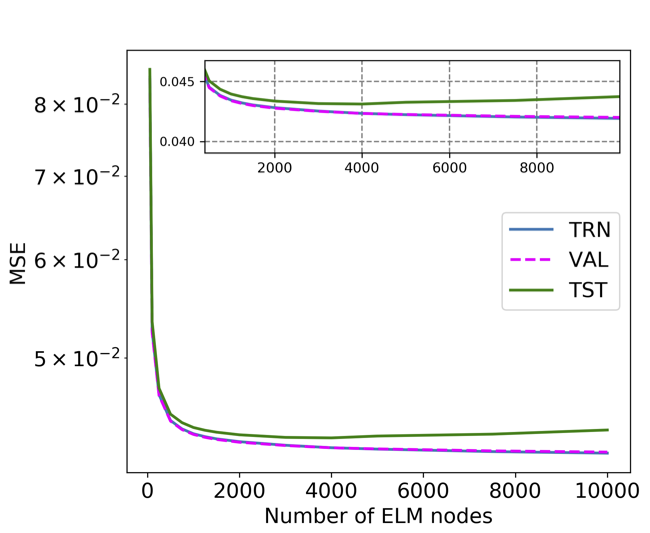
\includegraphics[width=\linewidth]{Figs/ELM_error.png}  
  \caption{}
  \label{figa:ELM_training}
\end{subfigure}
\begin{subfigure}{.49\textwidth}
  \centering
  % include first image
  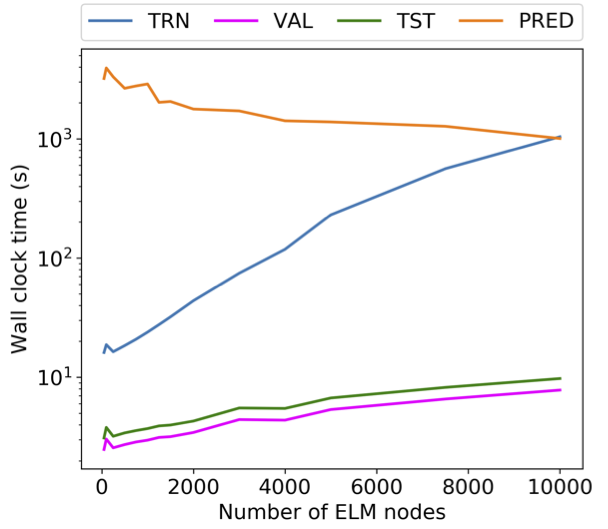
\includegraphics[width=\linewidth]{Figs/ELM_time.png}  
  \caption{}
  \label{figb:ELM_training}
\end{subfigure}
\caption{ELM tuning, including (a) wall clock time per model and (b) training (TRN), validation (VAL) and test (TST) MSE, both as a function of number of nodes.}
\label{fig:ELM_training}
\end{figure}

The tuning of ELM hyper-parameters based on the MSE minimization of the validation data (VAL) is performed by scanning $n$ ranging from 10 to 100 and $m$ from 50 to 10000. Preliminary studies showed that this is a reasonable range, given that higher values come at high computational cost without resulting in significant improvements. Depending on $m$, the wall clock time needed for training a single model can range from few seconds up to 15-20 minutes, as shown in Fig.~\ref{figa:ELM_training}, on a GPU accelerated machine using one K40 NVIDIA card. The optimal number of $n$ and $m$ is hence a trade-off between the computational time required by the model and the exhibited performance on the VAL sample.

The tuning procedure of $G_h$ for the month of June is visualised in Fig.~\ref{figa:ELM_training} and Fig.~\ref{figb:ELM_training}, while a numerical comparison of MSE, training and prediction times is provided in Table~\ref{tab:ELM_tuning}. The computational time (Fig.~\ref{figa:ELM_training}) is dominated by the evaluation of the chosen model on the dense spatial grid used for the GHI predictions (PRED). The MSE for VAL (Fig.~\ref{figb:ELM_training}), representing the model performance, steeply falls before 500 nodes and then stabilizes on low values without significant improvement when further increasing $m$, suggesting a minimum model size of $m = 500$. While the given data is for $G_h$ in June, similar trends exist for the other months, for $G_B$ and $\rho$. 
Considering also the computational time, which constantly increases with $m$, we choose the model hyper-parameters as a trade-off between performance and computational efficiency. 
The selected hyper-parameters are $m=1000, n=50$ for $G_h$ and $G_B$ and $m=1000, n=30$ for $\rho$.
The model performance on the test set (TST) shows a-posteriori that this choice is appropriate.

\begin{table}[tb]
\centering
\footnotesize
\caption{Results of the tuning of $m$, showing the trade-off between the validation MSE and training and prediction times (per ELM), for $G_h$ in June. The selected value for $m$ is shown in bold.}
\label{tab:ELM_tuning}

    \begin{tabular}{lccccccc}
    \hline
    \textit{m}          & 50    & 100   & 500   & \textbf{1000}  & 2000  & 5000  & 10000 \\ \hline
    Validation MSE      & 0.084 & 0.052 & 0.044 & \textbf{0.043} & 0.043 & 0.042 & 0.042 \\
    Training time (s)   & 16    & 18    & 18    & \textbf{23}    & 43    & 230   & 1040  \\
    Prediction time (s) & 2.5   & 3.0   & 2.7   & \textbf{3.0}   & 3.4   & 5.4   & 7.8   \\ \hline
    \end{tabular}
\end{table}

\subsection*{Random Forest}
\label{app:tune_RF}

Random Forests are used for two separate models, to estimate $C_{\mathit{pv}}$ (Section~\ref{panels}) and $C_{sh}$ (Section~\ref{shade}). Due to the smaller size of the data as compared to the ELM-E, a 5-fold cross-validation is applied. It splits the data into 5 subsets, from which 5 separate models are trained and validated each on a different subset. 
The RF has three main hyper-parameters which can be tuned: the number of trees in the ensemble ($n$), the minimum number of samples in each leaf node ($l$), and the number of features ($m$) which are randomly considered for splitting at each node. $m$ determines the level of randomization within each decision tree, $l$ impacts the level of smoothing of the predictions, while $n$ improves the robustness of the model, and is primarily limited by computational time \cite{breiman_random_2001}.
The selected hyper-parameters for both models are  $l = 3$, $m = 5$ and $n = 1000$. It should be noted that the RF is much less prone to small deviations in the model hyper-parameters than the ELM-E.

%%%%%%%%%%%%%%%%%%%%%%%%%%%%%%%%%%%%%%%%%%%%%%%%%%%%%%%

\section{Geospatial algorithms}

\subsection*{Virtual installation of PV panels}
\label{app:virtualPV}

Algorithm~\ref{alg:panels} details the geospatial algorithm that is implemented to virtually install PV panels on roof surfaces. It uses the python \texttt{geopandas} library \cite{kelsey_jordahl_geopandas/geopandas:_2019}. 
The output of the geospatial algorithm, $C_{\mathit{pv}}$, is calculated for each roof surface as the ratio between the roof area covered by $N_{\mathit{panels}}$ virtual panels, each of area $A_{\mathit{panel}}$, and the tilted area $A_{t}$ of the roof surfaces: 

\begin{equation}
\label{eq:cpv}
C_{\mathit{pv}} = \frac{N_{\mathit{panels}} \times A_{\mathit{panel}}}{A_t}
\end{equation}

\begin{algorithm}[htbp]
\caption{PV panel placement on rooftop polygons}
\label{alg:panels}
\begin{algorithmic}[1]
  \footnotesize
  \State Rotate roof surfaces to face south
  \State Create inside buffers (0.4m) along the roof edges
  \State Project PV panel dimensions for each tilted roof
  \Statex \textbf{for all} roof surfaces:
    \State \qquad Place rectangular grid on south-facing roof
    \State \qquad Remove grid cells (panels) outside roof surface
    \State \qquad Count panels and rotate to roof aspect
  \State Compute panelled area and panelled area ratio
\end{algorithmic}
\end{algorithm}

\subsection*{Shading effects}
\label{app:shade}

The shading effects, namely $S_{sh}$ and $C_{sh}$, are computed using horizon maps for each azimuth angle of the sun. Algorithm~\ref{alg:shade} describes the steps to extract $S_{sh}$ and $C_{sh}$ from the horizon maps.
The computation of these maps is the most computationally expensive step in the estimation of hourly RPV potential. Hence, several measures are taken to assure the feasibility of the approach:

\begin{enumerate}
    \item Horizon maps are computed in bins of $5^\circ$ for south-east to south-west sun azimuths (110-250$^\circ$), and in bins of $10^\circ$ for east (60-110$^\circ$) and west (250-300$^\circ$) azimuths, where solar radiation is low. Thus, only 38 maps need to be computed.
    \item The horizon distance is 100 m, i.e. a radius of 100 m is considered around each pixel to compute horizons. In Switzerland, where few high-rise buildings exist, this threshold is suitable to estimate the shading effects from surrounding trees and buildings.
    \item The algorithm is implemented using the GRASS GIS engine~\cite{neteler_grass_2012}. The Swiss terrain is split into 16 sub-regions and processed in parallel to reduce the computational time from $\sim$1000 to $\sim$30 hours. 
    
\end{enumerate}

\begin{algorithm}[htbp]
\caption{Computation of shading effects on rooftops}
\label{alg:shade}
\begin{algorithmic}[1]
  \footnotesize
  \State Compute horizon maps from DSM for 38 angle bins
  \State Crop horizon maps over (rasterized) roofs
  \Statex \textbf{for all} $t$:
    \State \qquad Apply binary filter to horizon maps using the solar position
  \State Average binary shading masks over \textit{t} (sun exposure map)
  \State Extract roof areas with sun exposure $< 40\%$
  \State Compute \textit{shaded area coefficient} $C_{sh}$
  \Statex \textbf{for all} $t$:
  	\State \qquad Extract roof areas with sun exposure $> 40\%$
    \State \qquad Compute \textit{hourly shading fraction} $S_{sh}(t)$
\end{algorithmic}
\end{algorithm}

\subsection*{Sky view factor}

The sky view factor is computed from similar horizon maps as described above for 32 equally spaced azimuth bins and a horizon distance of 100 m, using the \textit{skyview} add-on for GRASS GIS~\cite{zaksek_sky-view_2011}. The computation is performed in parallel over 64 sub-regions.

%%%%%%%%%%%%%%%%%%%%%%%%%%%%%%%%%%%%%%%%%%%%%%%%%%%%%%%

\section{Uncertainty propagation for tilted radiation}
\label{unc_Gt}

The variance and covariance of the three addends in Eq.~(\ref{eq:irrad}) (labelled $B, D, R$ in Eq.~(\ref{eq:irrad_unc})) are computed from the mean and variance of the horizontal radiation ($G_{B,D,h}$, $\sigma^2_{GB,GD,Gh}$), the partly shaded factor ($(1-S_{sh})$, $\sigma^2_{sh}$) and the sky view factor ($\mathit{SVF}$, $\sigma^2_{\mathit{SVF}}$) such that:

\begin{equation}
\begin{aligned}
% Definition of variance of beam component
\sigma^2_{B} & = F_{B}^2 (\sigma^2_{\mathit{Ssh}} G_B^2 + \sigma^2_{GB} (1-S_{sh})^2 + \sigma^2_{\mathit{Ssh}} \sigma^2_{GB}) \\
% Definition of variance of diffuse component     
\sigma^2_{D} & = F_{D}^2 (\sigma^2_{\mathit{SVF}} G_D^2 + \sigma^2_{GD} \mathit{SVF}^2 + \sigma^2_{\mathit{SVF}} \sigma^2_{GD}) \\
% Definition of variance of reflected component
\sigma^2_{R}&  = F_{R}^2 \sigma^2_{Gh}
\end{aligned}
\end{equation}

where $F_{B}, F_{D}, F_{R}$ are the beam, diffusion and reflection factors introduced in Eq.~\ref{eq:tilted_irrad_simplified}. 
Under the assumptions in Section~\ref{unc_prop}, we derive the covariances between the beam, diffuse and reflected components of $G_t$ as a function of the covariances between the horizontal radiation components, as well as the covariance between the shading and the SVF, such that:

\begin{equation}
\begin{aligned}
% covariance between direct and diffuse
\mathrm{Cov}(B, D) & = F_{B}  F_{D} \times (\mathrm{Cov}(G_B, G_D) \times \mathrm{Cov}(S_{sh}, \mathit{SVF}) \\
& + G_B  G_D \times \mathrm{Cov}(S_{sh}, \mathit{SVF}) \\
& + (1-S_{sh}) \times \mathit{SVF} \times \mathrm{Cov}(G_B, G_D)) \\
% covariance between direct and reflected
\mathrm{Cov}(B, R) & = F_{B}  F_{R} \times (1-S_{sh}) \times \mathrm{Cov}(G_B, G_h) \\
% covariance between diffuse and reflected
\mathrm{Cov}(D, R) & = F_{D}  F_{R} \times \mathit{SVF}  \times      \mathrm{Cov}(G_D, G_h) 
\end{aligned}
\end{equation}

where the covariances $\mathrm{Cov}(G_h, G_D)$ and $\mathrm{Cov}(G_B, G_D)$ are computed from $\sigma_{Gh}, \sigma_{GB}$ and $\sigma_{GD}$ in analogy to Eq.~(\ref{eq:unc_GD}).